% DO NOT COMPILE THIS FILE DIRECTLY!
% This is included by the other .tex files.

\begin{frame}[t,plain]
\titlepage
\end{frame}

\begin{frame}
    \frametitle{Outline of the presentation}
    \begin{itemize}
        \item Present the components used in MISP to expire IOCs
        \item Present the current state of Indicators life-cycle management in MISP
        \item Present the current state of Indicators life-cycle management in MISP
    \end{itemize}
\end{frame}

\section{Expiring IOCs: Why and How?}
\begin{frame}[fragile]
\frametitle{Indicators - Problem Statement}
    \begin{itemize}
        \item {\bf Sharing information} about threats {\bf is crucial}
        \item Organisations are sharing more and more
    \end{itemize}
    \vspace{1em}

    Contribution by {\bf unique organisation} (\texttt{Orgc.name}) on MISPPriv:\\
    \vspace{1em}
    \begin{minipage}{0.45\textwidth}
        \begin{tabular}{ll}
            \hline
            Date  & Unique Org \\
            \hline
            2013  & 17 \\
            2014  & 43 \\
            2015  & 82 \\
            2016  & 105 \\
            2017  & 118 \\
            2018  & 125 \\
            2019-10 & 135 \\
            \hline
        \end{tabular}
        \vspace{0.5em}
    \end{minipage}
    \begin{minipage}{0.5\textwidth}
        \begin{lstlisting}
{
    "distribution": [1, 2, 3]
}\end{lstlisting}
    \end{minipage}

\end{frame}

\begin{frame}
\frametitle{Indicators - Problem Statement}
    \begin{itemize}
        \item Various users and organisations can share data via MISP, multiple parties can be involved
        \begin{itemize}
            \item \textbf{Trust}, \textbf{data quality} and \textbf{time-to-live} issues
            \item Each user/organisation has \textbf{different use-cases} and interests
                \begin{itemize}
                    \item Conflicting interests such as operational security, attribution,... (depends on the user)
                \end{itemize}
        \end{itemize}
        \item[] $\rightarrow$ Can be partially solved with \textit{Taxonomies}
        \pause
        \vspace{0.5cm}
        \item Attributes can be shared in large quantities (more than 7.3 million on \texttt{MISPPRIV})
        \begin{itemize}
            \item Partial info about their \textbf{freshness} (\textit{Sightings})
            \item Partial info about their \textbf{validity} (last update)
        \end{itemize}
        \item[] $\rightarrow$ Can be partially solved with our \textit{Decaying model}
    \end{itemize}
\end{frame}

\begin{frame}
\frametitle{Requirements to enjoy the decaying feature in MISP}
        \begin{itemize}
            \item Starting from \textbf{MISP 2.4.116}, the decaying feature is available
            \item Don't forget to \textbf{update the decay models} and \textbf{enable} the ones you want
            \item The decaying feature has no impact on the information in MISP, it's just an \textbf{overlay} to be used in the user-interface and API
            \item Decay strongly relies on \textit{Taxonomies} and \textit{Sightings}, don't forget to review their configuration
        \end{itemize}
\end{frame}

\begin{frame}
    \frametitle{\textit{Sightings} - Refresher}
    \textit{Sightings} add \textbf{temporal context} to indicators.
    A user, script or an IDS can extend the information related to indicators by reporting back to MISP that
    an indicator has been \texttt{seen}, or that an indicator can be considered as a \texttt{false-positive}
    \vspace{0.5cm}
    \begin{itemize}
        \item \textit{Sightings} give more credibility/visibility to indicators
        \item This information can be used to {\bf prioritise and decay indicators}
    \end{itemize}
    \begin{center}
        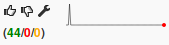
\includegraphics[scale=1.00]{pics/sightings.png}
    \end{center}
\end{frame}

\begin{frame}
    \frametitle{Taxonomies - Refresher (1)}
    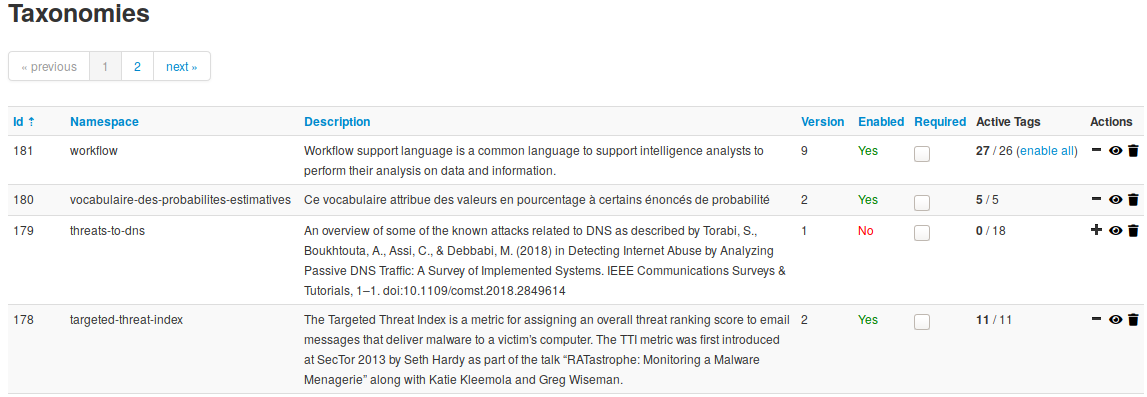
\includegraphics[width=1.00\linewidth]{pics/taxonomies.png}
    \begin{itemize}
        \item \textit{Taxonomies} are a simple way to attach a classification to an \textit{Event} or an \textit{Attribute}
        \item Classification must be globally used to be efficient (or agreed on beforehand)
    \end{itemize}
\end{frame}

\begin{frame}
    \frametitle{Taxonomies - Refresher (2)}
    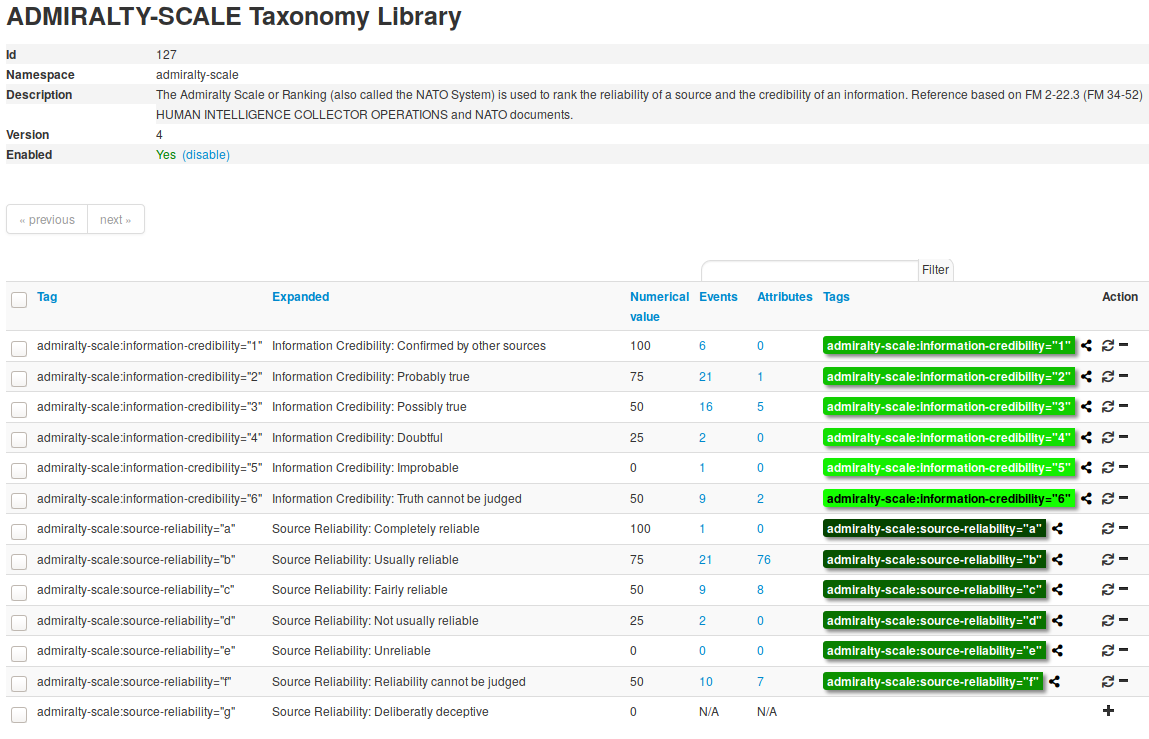
\includegraphics[width=1.00\linewidth]{pics/taxonomy-admiralty-scale.png}
    \begin{center}
        $\rightarrow$ Cherry-pick allowed \textit{Tags}
    \end{center}
\end{frame}

\begin{frame}
    \frametitle{Taxonomies - Refresher (3)}
    \begin{itemize}
        \item Some taxonomies have \texttt{numerical\_value}
        \begin{itemize}
            \item[$\rightarrow$] Can be used to prioritise \textit{Attributes}
        \end{itemize}
    \end{itemize}
    \vspace{0.5cm}

    \begin{footnotesize}
    \begin{columns}[T] % align columns
    \begin{column}{.40\textwidth}
        \begin{tabular}{|ll|}
            \hline
            \textbf{Description} & \textbf{Value}\\
            \hline
            Completely reliable & 100\\
            Usually reliable & 75\\
            Fairly reliable & 50\\
            Not usually reliable & 25\\
            Unreliable & 0\\
            Reliability cannot be judged & 50 \textbf{\color{red}?}\\
            Deliberatly deceptive & 0 \textbf{\color{red}?}\\
            \hline
        \end{tabular}
    \end{column}%
    \hfill%
    \begin{column}{.48\textwidth}
        \begin{tabular}{|ll|}
            \hline
            \textbf{Description} & \textbf{Value}\\
            \hline
            Confirmed by other sources & 100\\
            Probably true & 75\\
            Possibly true & 50\\
            Doubtful & 25\\
            Improbable & 0\\
            Truth cannot be judged & 50 \textbf{\color{red}?}\\
            \hline
        \end{tabular}
    \end{column}%
    \end{columns}
    \end{footnotesize}

    \vspace{0.5cm}
    $\rightarrow$ In next version, Users will be able to override these \texttt{numerical\_value}
\end{frame}

\begin{frame}
    \frametitle{Scoring Indicators: Our solution}
    $$ \texttt{score}(\texttt{\tiny Attribute}) = \texttt{base\_score}(\texttt{\tiny Attribute, Model}) \;\;\bullet\;\; \texttt{decay}(\texttt{\tiny Model, time}) $$
    Where,\vspace{0.5cm}
    \begin{itemize}
        \item \texttt{score} $ \in [0, +\infty $
        \item \texttt{base\_score} $ \in [0, 100] $
        \item \texttt{decay} is a function defined by model's parameters controlling decay speed
        \item \texttt{Attribute} Contains \textit{Attribute}'s values and metadata {\scriptsize (\textit{Taxonomies}, \textit{Galaxies}, ...)}
        \item \texttt{Model} Contains the \textit{Model}'s configuration
    \end{itemize}
    
\end{frame}

\begin{frame}
    \frametitle{Scoring Indicators: Our solution}
    $$ \texttt{score}(\texttt{\tiny Attribute}) = \texttt{base\_score}(\texttt{\tiny Attribute, Model}) \;\;\bullet\;\; \texttt{decay}(\texttt{\tiny Model, time}) $$
    \begin{itemize}
        \item \texttt{base\_score}(\texttt{\tiny Attribute, Model})
            \begin{itemize}
                \item Initial score of the \textit{Attribute} only considering the context (i.e. \textit{Tags})
            \end{itemize}
        \vspace{1cm}
        \item \texttt{decay}(\texttt{\tiny Model, time})
            \begin{itemize}
                \item Function composed of the \textbf{lifetime} and \textbf{Decay speed} decreasing the \texttt{base\_score} over time
            \end{itemize}
    \end{itemize}
\end{frame}

\section{Current implementation in MISP}
\begin{frame}
    \frametitle{Implementation in MISP: \texttt{Event/view}}
    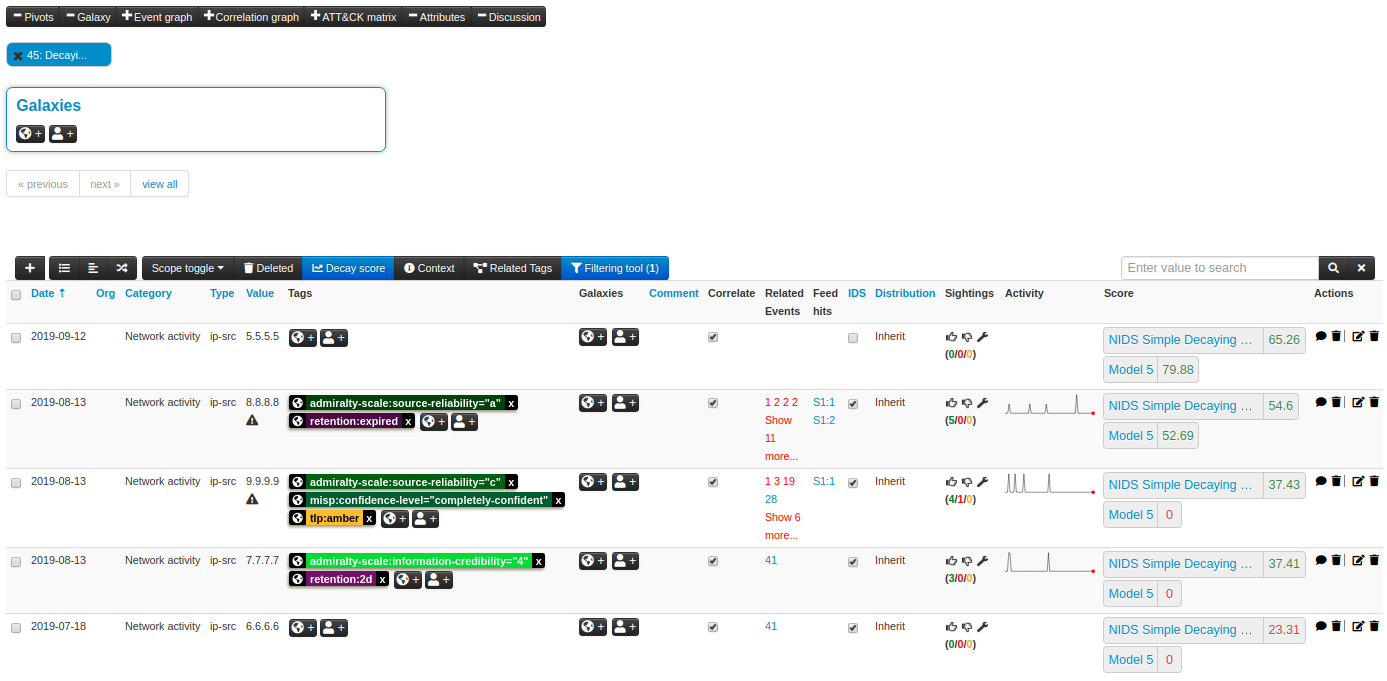
\includegraphics[width=1.00\linewidth]{pics/decaying-event.png}
    \begin{itemize}
        \item \texttt{Decay score} toggle button
        \begin{itemize}
            \item Shows Score for each \textit{Models} associated to the \textit{Attribute} type
        \end{itemize}
    \end{itemize}
\end{frame}

\begin{frame}[fragile]
    \frametitle{Implementation in MISP: API result}
    \texttt{/attributes/restSearch}
    \begin{lstlisting}
"Attribute": [
  {
    "category": "Network activity",
    "type": "ip-src",
    "to_ids": true,
    "timestamp": "1565703507",
    [...]
    "value": "8.8.8.8",
    "decay_score": [
      {
        "score": 54.475223849544456,
        "decayed": false,
        "DecayingModel": {
          "id": "85",
          "name": "NIDS Simple Decaying Model"
        }
      }
    ],
[...]
    \end{lstlisting}
\end{frame}

\begin{frame}
\frametitle{Implementation in MISP: Objectives}
    \begin{itemize}
        \item \textbf{Automatic scoring} based on default values
        \item \textbf{User-friendly UI} to manually set \textit{Model} configuration (lifetime, decay, etc.)
        \item \textbf{Simulation} tool
        \item Interaction through the \textbf{API}
        \item Opportunity to create your \textbf{own} formula or algorithm
    \end{itemize}
\end{frame}

\begin{frame}
    \frametitle{Implementation in MISP: Models definition}
        \hspace{190pt}
        \raisebox{-1.0ex}{\Large $\Rsh$} {\tiny $score = base\_score \cdot \left( 1 - \left( \frac{t}{\tau} \right)^{\frac{1}{\delta}} \right) $}
    \textit{Models} are an instanciation of the formula where elements can be defined:
    \begin{itemize}
        \item Parameters: \texttt{lifetime, decay\_rate, threshold}
        \item \texttt{base\_score}
        \item \texttt{default base\_score}
        \item formula
        \item associate \textit{Attribute} types
        \item creator organisation
    \end{itemize}
\end{frame}

\begin{frame}
    \frametitle{Implementation in MISP: Models Types}
    Multiple model types are available
    \begin{itemize}
        \item \textbf{Default Models}: Models created and shared by the community. Available from \texttt{misp-decaying-models} repository\footnote{\url{https://github.com/MISP/misp-decaying-models.git}}.
        \begin{itemize}
            \item $\rightarrow$ Not editable
        \end{itemize}
    \item \textbf{Organisation Models}: Models created by a user belonging to an organisation
        \begin{itemize}
            \item These models can be hidden or shared to other organisation 
            \item $\rightarrow$ Editable
        \end{itemize}
    \end{itemize}
\end{frame}

\begin{frame}
    \frametitle{Implementation in MISP: Index}
    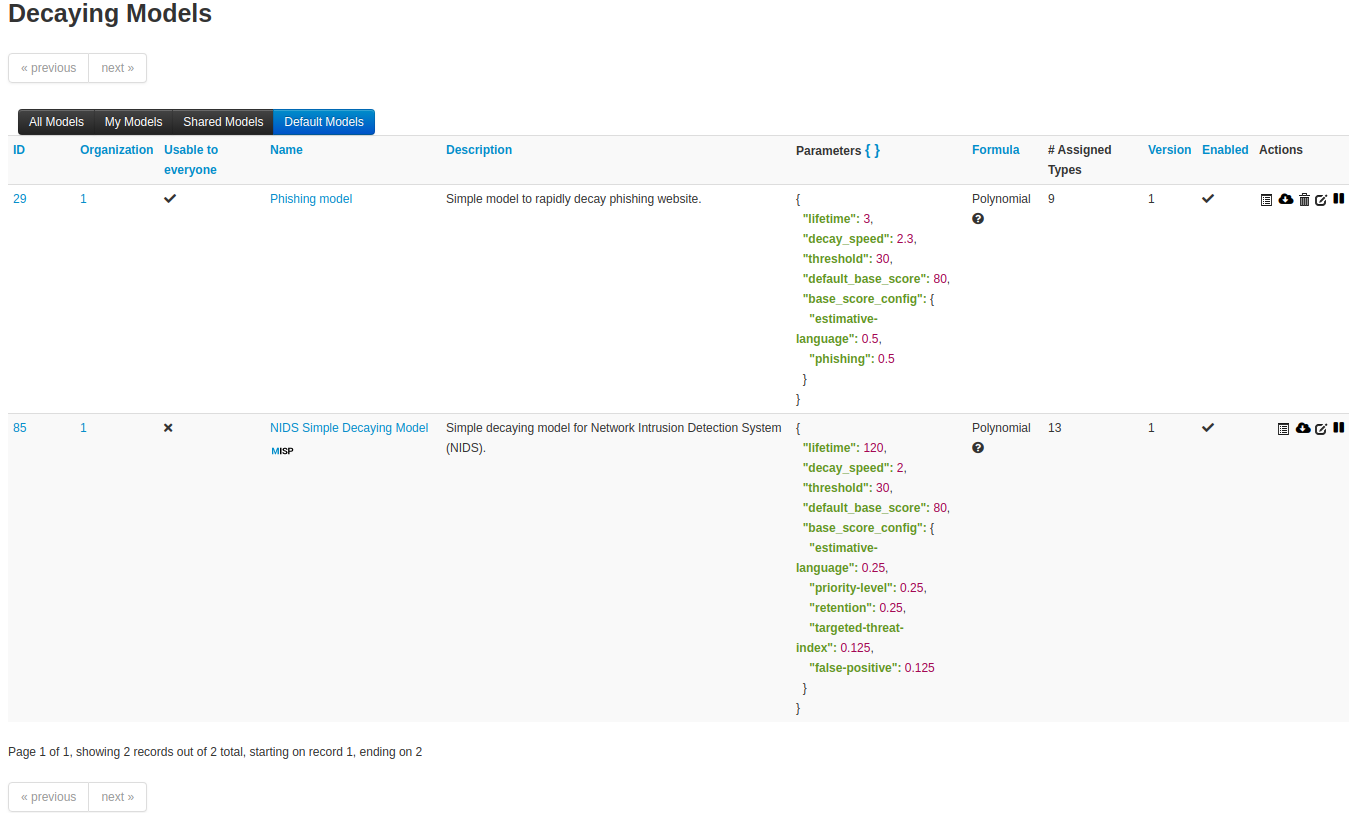
\includegraphics[width=1.00\linewidth]{pics/decaying-index.png}
    View, update, add, create, delete, enable, export, import
\end{frame}

\begin{frame}
    \frametitle{Implementation in MISP: Fine tuning tool}
    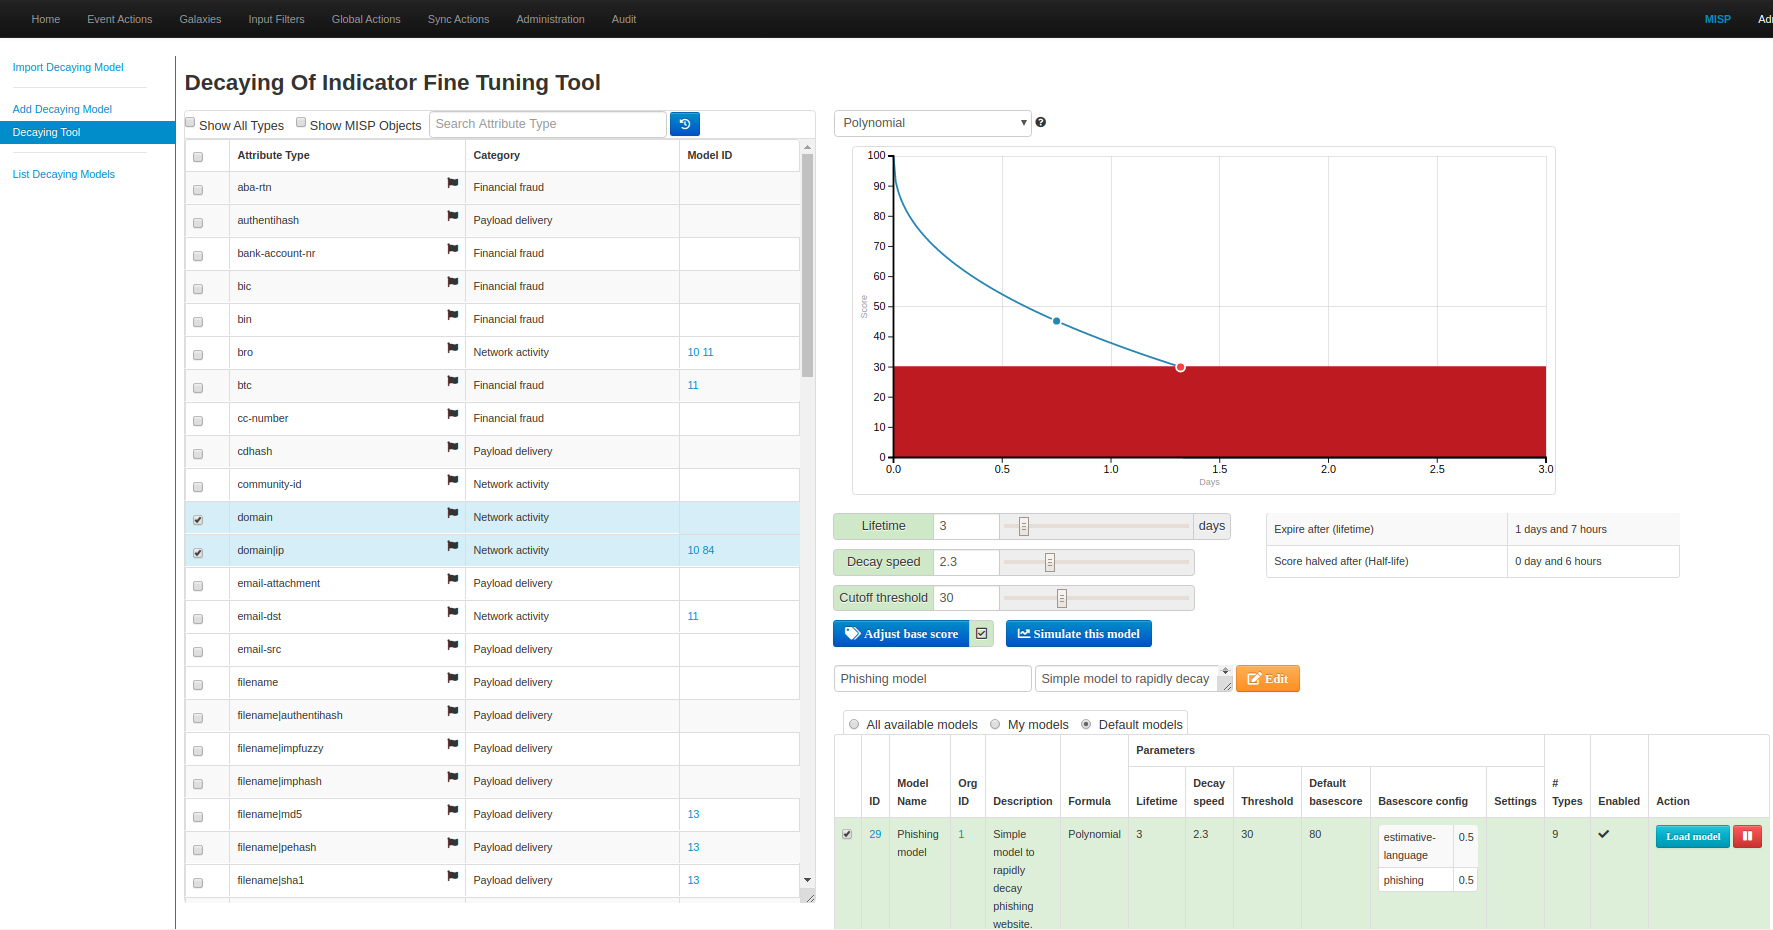
\includegraphics[width=1.00\linewidth]{pics/decaying-tool.png}
    Create, modify, visualise, perform mapping
\end{frame}

\begin{frame}
    \frametitle{Implementation in MISP: \texttt{base\_score} tool}
    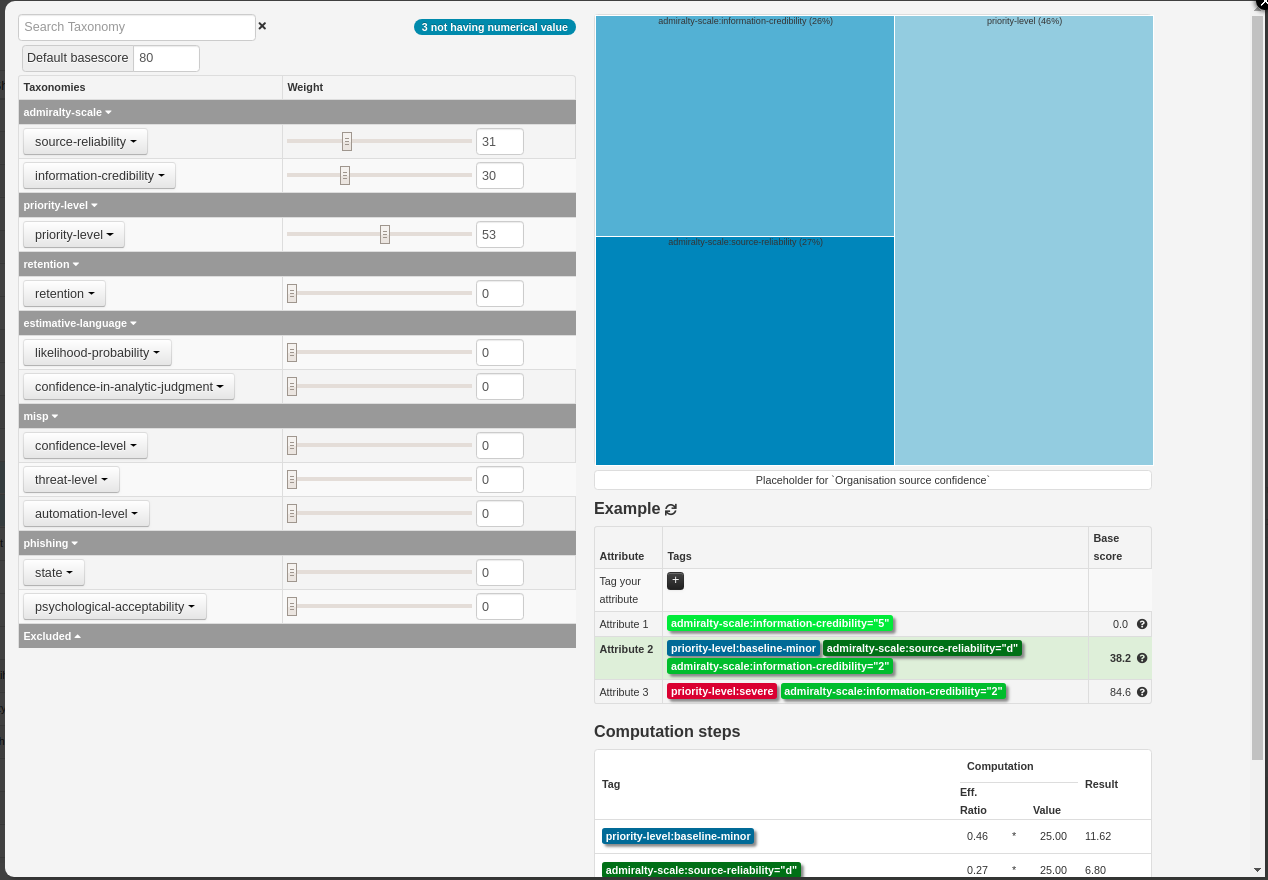
\includegraphics[width=1.00\linewidth]{pics/decaying-basescore.png}
    Adjust Taxonomies relative weights
\end{frame}

\begin{frame}
    \frametitle{Implementation in MISP: simulation tool}
    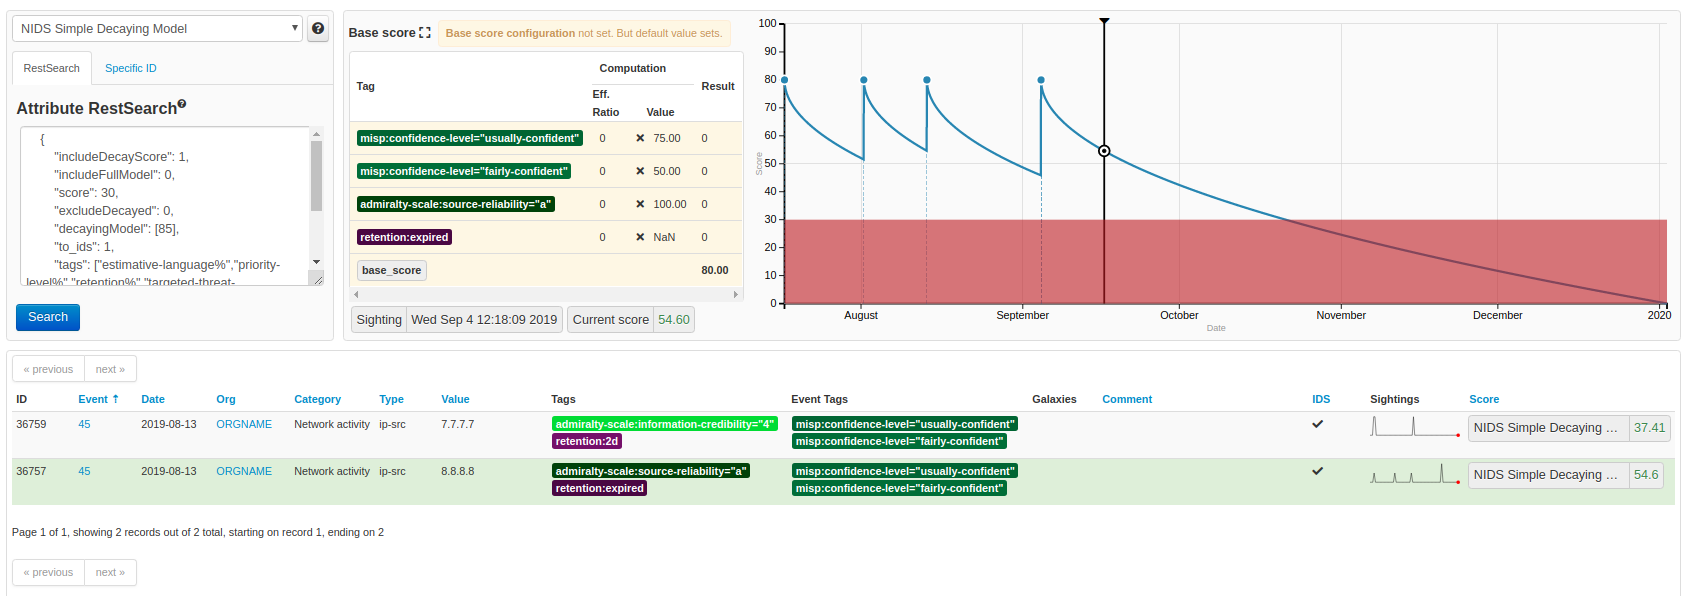
\includegraphics[width=1.00\linewidth]{pics/decaying-simulation.png}
    Simulate \textit{Attributes} with different \textit{Models}
\end{frame}

\begin{frame}[fragile]
    \frametitle{Implementation in MISP: API query body}
    \texttt{/attributes/restSearch}
    \begin{lstlisting}
{
    "includeDecayScore": 1,
    "includeFullModel": 0,
    "excludeDecayed": 0,
    "decayingModel": [85],
    "modelOverrides": {
        "threshold": 30
    }
    "score": 30,
}
    \end{lstlisting}
\end{frame}

\lstset{language=PHP}
\begin{frame}[fragile]
    \frametitle{Creating a new decay algorithm}
    \lstset{basicstyle=\scriptsize}
    \begin{lstlisting}
<?php
include_once 'Base.php';

class Polynomial extends DecayingModelBase
{
    public const DESCRIPTION = 'The description of your new decaying algorithm';

    public function computeScore($model, $attribute, $base_score, $elapsed_time)
    {
       // algorithm returning a numerical score
    }

    public function isDecayed($model, $attribute, $score)
    {
        // algorithm returning a boolean stating
        // if the attribute is expired or not
    }
}
?>
    \end{lstlisting}
\end{frame}

\begin{frame}
    \frametitle{Decaying Models 2.0}
    \begin{itemize}
        \item Improved support of \textit{Sightings}
        \begin{itemize}
            \item \texttt{False positive} \textit{Sightings} should somehow reduce the score
            \item \texttt{Expiration} \textit{Sightings} should mark the attribute as decayed
        \end{itemize}
        \item Potential \textit{Model} improvements
        \begin{itemize}
            \item Instead of resetting the score to \texttt{base\_score} once a \textit{Sighting} is set, the score should be increased additively (based on a defined coefficient); thus \textbf{prioritizing surges} rather than infrequent \textit{Sightings}
            \item Take into account related \textit{Tags} or \textit{Correlations} when computing score
        \end{itemize}
        \item Increase \textit{Taxonomy} coverage
        \begin{itemize}
            \item Users should be able to manually override the \texttt{numerical\_value} of \textit{Tags}
        \end{itemize}
    \end{itemize}
\end{frame}
